\documentclass[12pt,letterpaper]{article}
\usepackage{fullpage}
\usepackage[top=2cm, bottom=4.5cm, left=2.5cm, right=2.5cm]{geometry}
\usepackage{amsmath,amsthm,amsfonts,amssymb,amscd}
\usepackage{lastpage}
% \usepackage{hyperref}
\usepackage{enumerate}
\usepackage{fancyhdr}
\usepackage{mathrsfs}
\usepackage{xcolor}
\usepackage{graphicx}
\usepackage{listings}
%\usepackage{mcode}
%\usepackage{hyperref}
\usepackage{movie15}
\usepackage{float}


\usepackage[colorlinks = true,
            linkcolor = blue,
            urlcolor  = blue,
            citecolor = blue,
            anchorcolor = blue]{hyperref}

% load package with ``framed'' and ``numbered'' option.
\usepackage[framed,numbered,autolinebreaks,useliterate]{mcode}

% \hypersetup{%
%   colorlinks=true,
%   linkcolor=blue,
%   linkbordercolor={0 0 1}
% }
 
% \renewcommand\lstlistingname{Algorithm}
% \renewcommand\lstlistlistingname{Algorithms}
% \def\lstlistingautorefname{Alg.}

% \lstdefinestyle{Python}{
%     language        = Python,
%     frame           = lines, 
%     basicstyle      = \footnotesize,
%     keywordstyle    = \color{blue},
%     stringstyle     = \color{green},
%     commentstyle    = \color{red}\ttfamily
% }

\setlength{\parindent}{0.0in}
\setlength{\parskip}{0.05in}

% Edit these as appropriate
\newcommand\course{Digital Signal Processing}
\newcommand\hwnumber{2}                  % <-- homework number
\newcommand\NetIDa{Mehdi Raza Khorasani}           % <-- NetID of person #1
\newcommand\NetIDb{}           % <-- NetID of person #2 (Comment this line out for problem sets)

\pagestyle{fancyplain}
\headheight 35pt
\lhead{\NetIDa}
\lhead{\NetIDa\\\NetIDb}                 % <-- Comment this line out for problem sets (make sure you are person #1)
\chead{\textbf{\Large Homework \hwnumber}}
\rhead{\course \\ \today}
\lfoot{}
\cfoot{}
\rfoot{\small\thepage}
\headsep 1.5em

\begin{document}

\section*{Question 1}
\subsection*{Part (a)}
From the definition of Z-Transform: 
\[
    X(z)= \sum_{n=-\infty}^{\infty} x(n)z^{-n}
\]
So we get: 
\[
    X(z) = (3)z^{-3} + (0)z^{-2} + (0)z^{-1} + (6)z^{0} + (1)z^{1} + (-4)z^{2}
\]
\[
\boxed{
X(z) = 3z^{-3} +  6 + z  -4z^{2}
}
\]

\subsection*{Part (b)}
\begin{figure}[h]
    \centering
    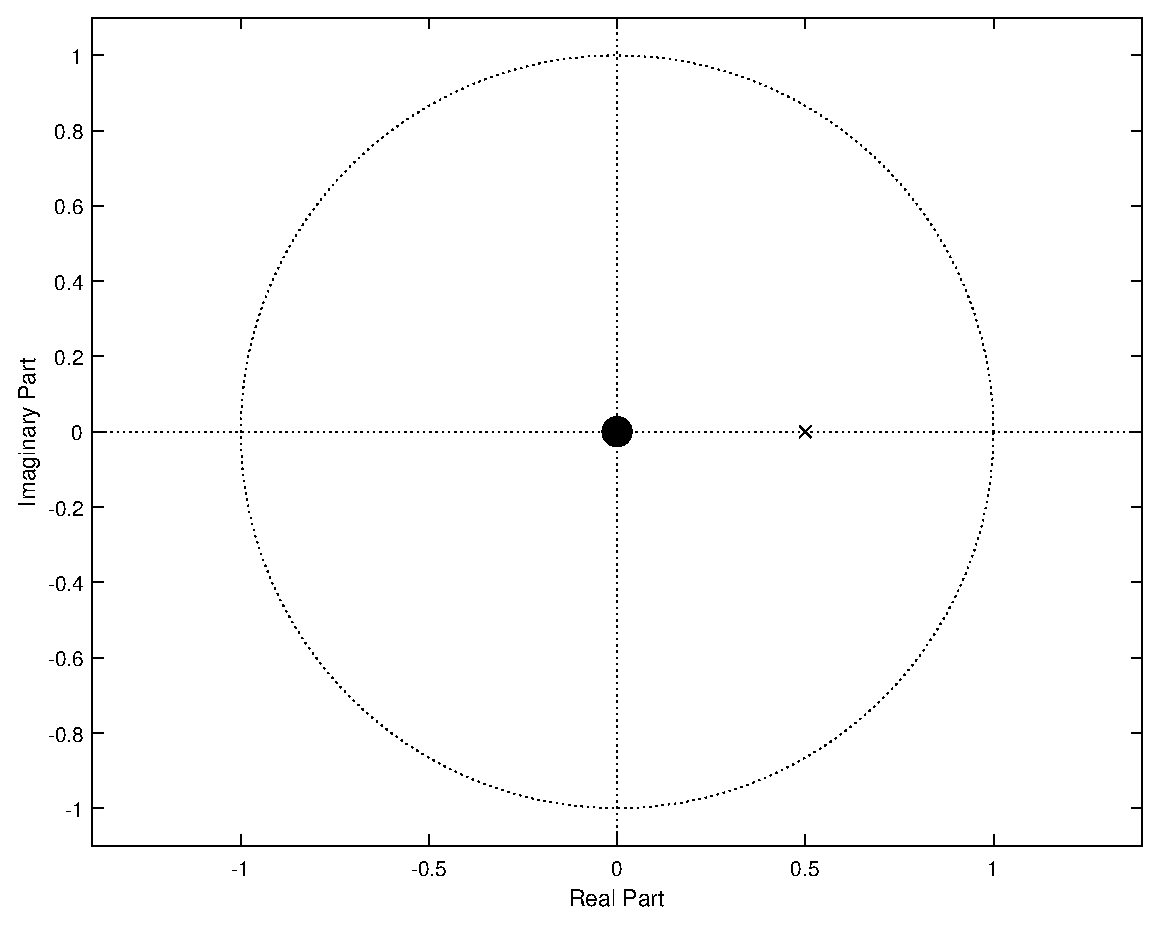
\includegraphics[scale=0.5]{figures/q1task2.eps}
    \caption{PZ plot for Q1}
    \label{PZq1}
\end{figure}
\subsubsection*{Proof 1}
We know that if system is FIR, then it is non-recursively and defined as follows: 
\[
    y(n)=\sum^{\infty}_{k=-\infty} b_k x(n-k)
\]
Taking Z-transform, we get: 
\[
    Y(z) = \sum^{\infty}_{k=-\infty} b_k X(z)z^{-k}
\]
From above equation, we can observe the following constraint for FIR system: 
\begin{enumerate}
    \item It can contain any number of zeros. 
    \item It does not contain any poles.
    \item Its ROC will be the whole z plane (due to absense of poles).
\end{enumerate}
Since the given system violates the condition 2 and 3, it is not FIR. So it  can be safely termed \textbf{IIR}.
\subsubsection*{Proof 2}
We have: 
\[
    H(z) = G z^{N-M} \dfrac{\prod_{k=1}^{M} (z-z_k)}{\prod_{k=1}^N (z-p_k)}
\]
where $G = \dfrac{b_o}{a_o}$.\\
In our case: 
\[
    N=M=1
\]
Then: 
\[
    H(z) = G z^0 \dfrac{z}{z-0.5}
\]
\[
    H(z) = G \dfrac{z}{z-0.5}
\]
We know that: 
\[
    H(z) = \dfrac{Y(z)}{X(z)}
\]
So the system function can be written as: 
\[
    \dfrac{Y(z)}{X(z)} = \dfrac{b_o}{a_o} (\dfrac{z}{z-0.5})
\]
Multiply and divide by $z^{-1}$:
\[
    \dfrac{Y(z)}{X(z)} = \dfrac{b_o}{a_o} (\dfrac{1}{1-0.5z^{-1}})
\]
Re-arranging: 
\[
    a_o Y(z) - 0.5a_oY(z)z^{-1} = b_o X(z) 
\]
Converting to LCCDE form: 
\[
    a_o y(n) - 0.5 a_o y(n-1) = b_o x(n-1)
\]
\[
\boxed{
    a_o y(n) = 0.5 a_o y(n-1) + b_o x(n-1)
}
\]
The given LCCDE is recursively defined hence the system is indeed IIR. Verified!
\pagebreak
\section*{Question 2}
Given: 
\[
    y(n) = 0.8 y(n-1)-0.6y(n-2) + x(n)+ 2x(n-1)
\]
\subsection*{Part (a)}
Taking Z-Transform on both sides: 
\[
    Y(z) = 0.8 z^{-1}Y(z) -0.6Y(z) z^{-2} + X(z) + 2X(z) z^{-1}
\]
\[
    Y(z)(1+0.6z^{-2} - 0.8z^{-1}) =  X(z)(1+2z^{-1})
\]
\[
    \dfrac{Y(z)}{X(z)} = \dfrac{1+2z^{-1}}{1-0.8z^{-1} + 0.6z^{-2}}
\]
\[
    = \dfrac{z^2 + 2z}{z^2-0.8z + 0.6}
\]
\[
    H(z) = \dfrac{z(z + 2)}{z^2-0.8z + 0.6}
\]

\subsection*{Part (b)}
\subsubsection*{Zeros}
Zeros are as follows: 
\[
    z = 0
\]
\[
    z=-2
\]
\subsubsection*{Poles}
Calculating roots of the equation below: 
\[
    z^2-0.8z+0.6 = 0
\]
Poles are as follows: 
\[
    p = 0.4 + 0.6633j
\]
\[
    p = 0.4 - 0.6633j
\]
\begin{figure}[h]
    \centering
    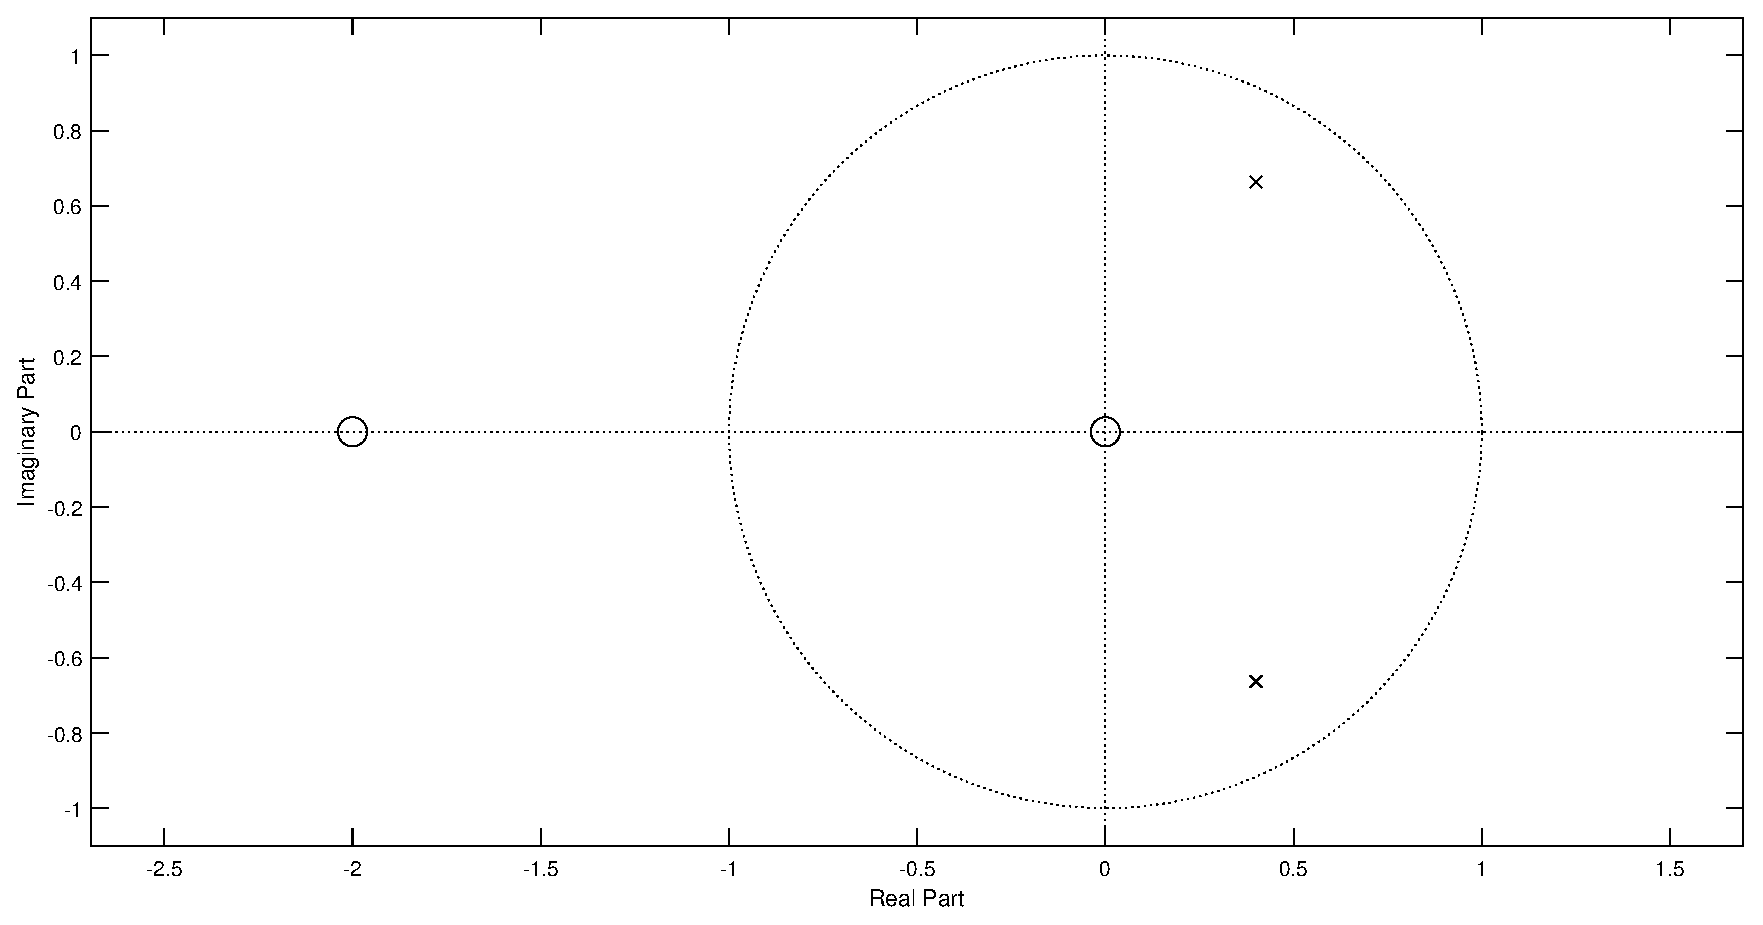
\includegraphics[scale=0.5]{figures/q2task3.eps}
    \caption{PZ plot}
    \label{PZq2}
\end{figure}
\subsection*{Part (c)}
The outer most pole is located at: 
\[
    r = \sqrt{0.4^2 +0.6633^2} = 0.7746
\]
Since system is causal, the ROC consists of $r>0.7746$. This implies that the ROC will include the unit circle (we may also observe this from the PZ plot). So system is stable. 
\pagebreak
\section*{Question 3}
Given: 

\[
    H(z) = \dfrac{z^2+z}{z^2+z-0.75}
\]
\subsection*{Part (a)}
\begin{figure}[!h]
    \centering
    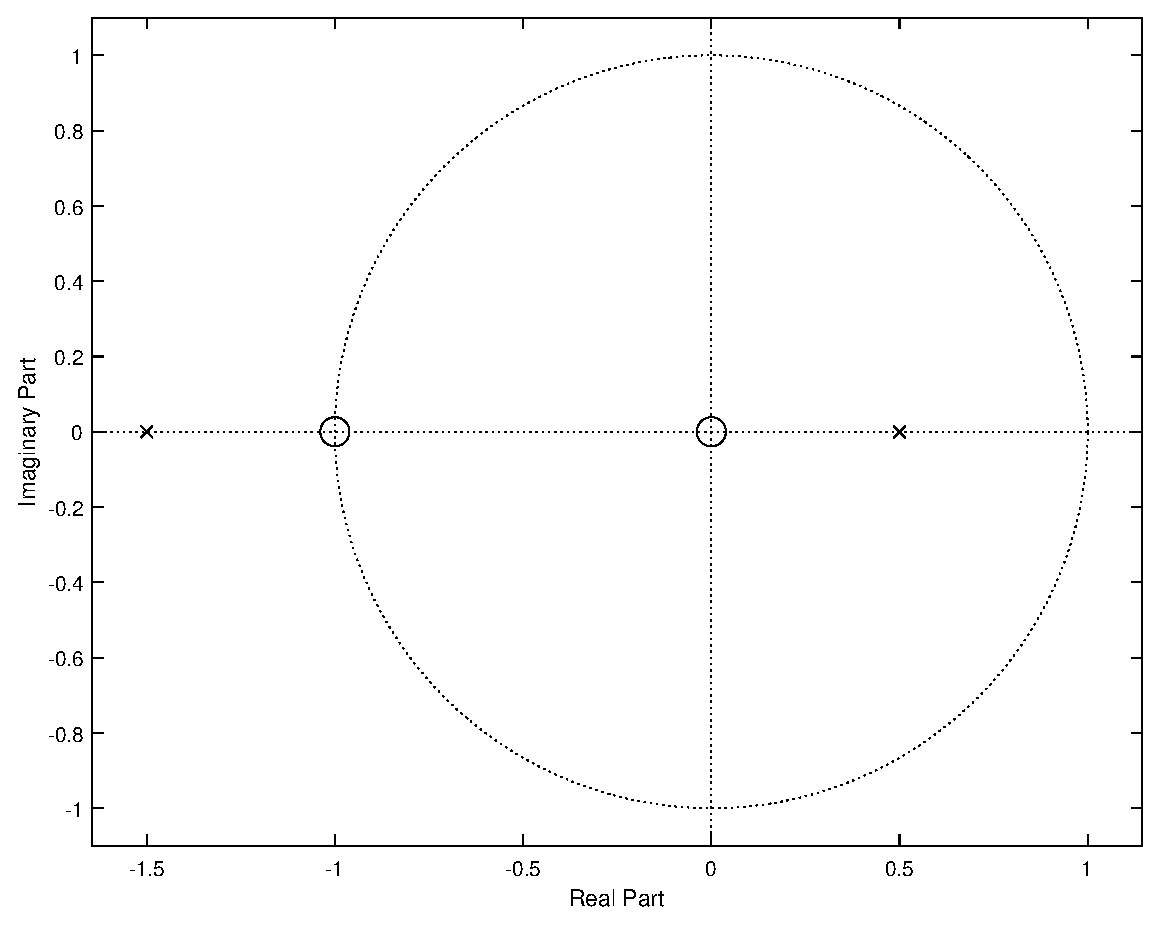
\includegraphics[scale=0.5]{figures/q3task1.eps}
    \caption{PZ plot for Q3}
    \label{PZq3}
\end{figure}
\subsubsection*{Zeros}
Zeros are calculated as follows: 
\[
    z(z+1) = 0
\]
Then, 
\[
\boxed{
z = 0
}
\]
\[
    \boxed{
    z = -1
    }
\]
\subsubsection*{Poles}

Poles are calculated as follows: 
\[
    z^2+z-0.75 = 0 
\]
\[
\boxed{
p = -1.5
}
\]
\[
\boxed{
p = 0.5
}
\]

\subsection*{Part (b)}
The outer most pole lies at: 
\[
    r = 1.5
\]
With the system obeying causality, its ROC will be $r>1.5$. So ROC doesn't includes the unit circle. So system is \textbf{unstable}

\subsection*{Part (c)}
The system function can be written as: 
\[
    \dfrac{Y(z)}{X(z)} = \dfrac{z^2+z}{z^2+z-0.75}
\]
Multiply and divide by $z^{-2}$
\[
    \dfrac{Y(z)}{X(z)} = \dfrac{1+z^{-1}}{1+z^{-1} - 0.75z^{-2}}
\]

\[
 Y(z) + Y(z)z^{-1} -0.75Y(z)z^{-2} = X(z) + X(z)z^{-1}    
\]
Above equation can now be converted into LCCDE form: 
\[
    y(n) + y(n-1) -0.75y(n-2) = x(n) + x(n-1) 
\]
\[
\boxed{
    y(n) = -y(n-1) +0.75y(n-2) + x(n) + x(n-1) 
}
\]
\pagebreak
\section*{Question 4}
Given: 
\[
    X(z) = \dfrac{z}{z^2+z-0.75}
\]
\[
    \dfrac{X(z)}{z} = \dfrac{1}{z^2+z-0.75}
\]
Creating partial fractions: 
\[
  \dfrac{1}{(z+1.5)(z-0.5)} = \dfrac{A_1}{(z+1.5)}  +\dfrac{A_2}{(z-0.5)}
\]
\[
 1 = A_1(z-0.5)+A_2(z+1.5)
\]
\subsection*{For $A_1$}
Put $z=-1.5$
\[
     1 = -2A_1  +0
\]
\[
\boxed{
A_1 = -0.5
}
\]
\subsection*{For $A_2$}
Put $z=0.5$
\[
     0.5 = 2A_2  +0
\]
\[
\boxed{
A_2 = 0.25
}
\]
Then Partial fraction expansion becomes: 
\[
\boxed{
  \dfrac{X(z)}{z} = \dfrac{-0.5}{(z+1.5)}  +\dfrac{0.25}{(z-0.5)}
}
\]
\[
    X(z) = \dfrac{-0.5z}{(z+1.5)}  +\dfrac{0.25z}{(z-0.5)}
\]
Multiply and divide by $z^{-1}$:
\[
    X(z) =  \dfrac{-0.5}{(1+1.5z^{-1})}  +\dfrac{0.25}{(1-0.5z^{-1})}
\]
From the lookup table, the inverse transform is given as: 
\[
\boxed{
    x(n) = [-0.5(-1.5)^n + 0.25( 0.5)^n] u(n)
}
\]
\pagebreak
\section*{Question 5}

\subsection*{Part (a)}
Since the fiter is high pass, we may place pole at $\omega = \pi$ and zero at $\omega = 0$. One possible arrangement is shown in the PZ plot:
\begin{figure}[h]
    \centering
    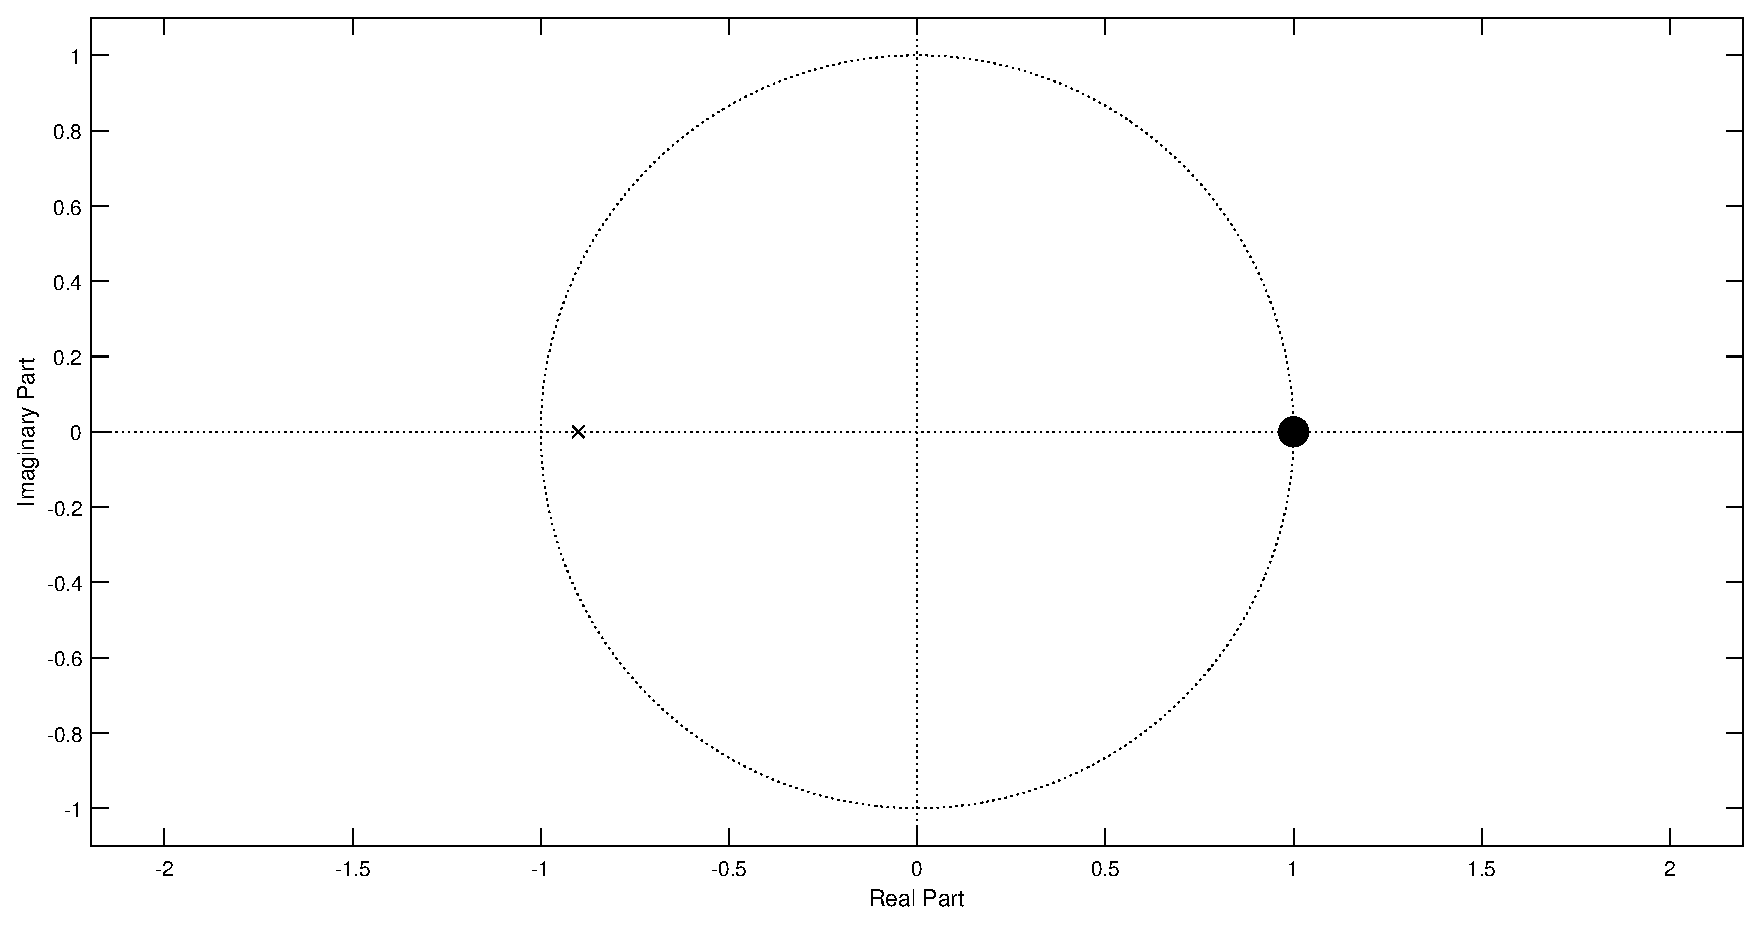
\includegraphics[scale=0.5]{figures/q5task1.eps}
    \caption{PZ plot for Q5}
    \label{PZq5}
\end{figure}
\subsection*{Part (b)}
\begin{enumerate}
    \item This is a band-pass filter for frequencies near $\omega=\pm \pi/ 2$. It is so because we see poles at frequency $\pm \pi/ 2$  (Poles are placed near frequencies to be emphasized). Similarly, we see zeros at $\omega = \pi $ and $\omega = 0$ (zeros are placed near frequencies to be de-emphasized). Hence this filter will block low and high frequencies ($\omega = 0 $ and $\omega = \pi$) and pass frequencies around $\omega = \pm \pi/ 2$. 
    \item 
    At $\omega =0$, the response is: 
    \[
     |H(\omega)| = b_o \dfrac{\textit{product of length of vector: zero to unit circle}}{\textit{product of length of vector: pole to unit circle}}
    \]
    Hence the response in this case will be (Assuming poles at $r = 0.9$): 
    \[
    |H(\omega)| = b_o \dfrac{1\times 1}{0.9 \times 0.9}
    \]
    \[
    |H(\omega)| =  1.234b_o
    \]
\end{enumerate}
\section*{Index}
The complete source code can be found at: \href{https://github.com/mehhdiii/Z-Transform-Basics}{GitHub/mehhdiii/}
\end{document}
